\chapter[Arranjo Físicos e Fluxo]{Arranjo Físicos e Fluxo}
\label{chap:arranjo}

	\section[Definição]{Definição}
	\label{sec:arranjo_definicao}

		O conceito de arranjo físico está ligeiramente ligado a forma física da cadeia de produção. Ou seja, o posicionamento físico dos recursos transformação. Neste sentido, ao definir um arranjo físico, está-se definindo a disposição física de onde serão colocados maquinas, pessoas, equipamentos, produtos etc.

		Visualmente, o arranjo físico possui diversas formas a depender do negócio tratado, mas quando a perspectiva é aérea, é possível nitidamente perceber como ocorre seu fluxo. Como ilustra a imagem a seguir.

		\begin{figure}[h]
			\centering
			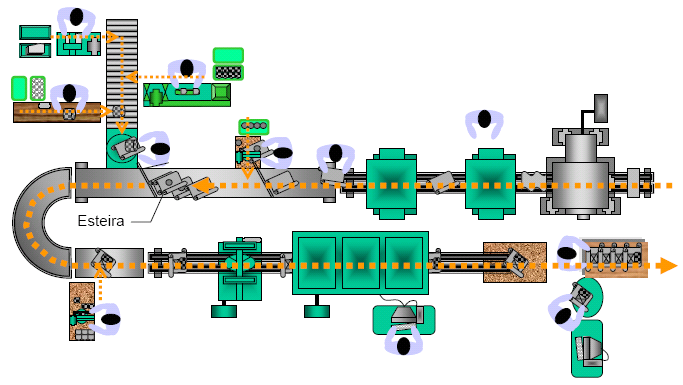
\includegraphics[scale=0.8]{arranjo1}
			\caption[Arranjo Físico Linear]{Arranjo Físico Linear. (Dr. Dario I. Miyake - PRO/EPUSP)}
			\label{fig:arranjo1}
		\end{figure}

		Existem razões práticas pelas quais as decisões de arranjo físico são importantes na maioria dos tipos de produção. São elas:

		\begin{enumerate}
			\item{Mudanças em um arranjo físico podem ser uma atividade difícil e longa por conta das dimensões físicas envolvidas nas maquinas e equipamentos;}
			\item{Rearranjo\footnote{Ato de remodelar um arranjo.} pode custar caro, pois sem um prévio planejamento, o processo de mudança pode interromper o funcionamento do serviço ou produção do produto levantado certamente a insatisfação dos clientes;}
			\item{No caso de um arranjo físico ser modelado de forma errônea, o fluxo poderá ser delongado, ou até mesmo gerar confusão, resultando em filas durante a produção, estoque desnecessário, recursos perdidos, entre outros.}
		\end{enumerate}

		De fato, gerenciar o arranjo físico de um produto ou serviço não é uma tarefa simples, exigindo um esforço para entendimento do processo de produção. A consequência de qualquer mau julgamento na definição do arranjo físico terá efeitos de longo prazo consideráveis na operação.

		Segundo \cite{slack}, “Projetar o arranjo físico de uma operação produtiva, assim como qualquer atividade de projeto, deve iniciar-se com os objetivos estratégicos da produção [...]”, isto é válido para qualquer processo de produção, entretanto isso é apenas o ponto de partida para um processo que possui diversas etapas no qual levam ao arranjo físico final de uma operação. Para isso, existe um processo bem definido de como chegar a um arranjo. A imagem a seguir ilustra esse processo.

		\begin{figure}[h]
			\centering
			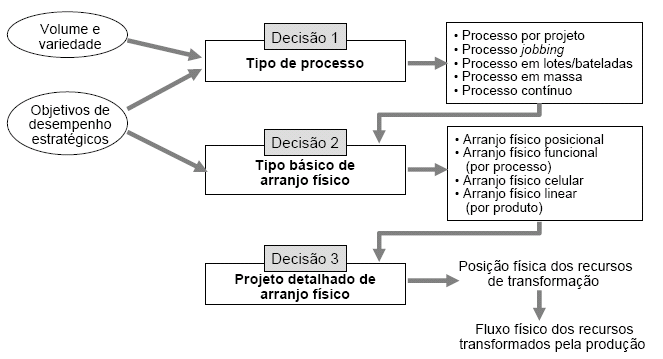
\includegraphics[scale=0.8]{arranjo2}
			\caption[Projeto de Arranjo Físico - Decisões a serem tomadas]{Projeto de Arranjo Físico - Decisões a serem tomadas. \cite{slack}}
			\label{fig:arranjo2}
		\end{figure}

		Para a primeira decisão é escolhido o tipo de processo do produto/serviço. Nesta etapa são definidas o binômio \textbf{volume-variedade}, isto é, o quanto será produzido e qual a sua diversidade de produtos. Essas duas características são fundamentais para suporte a segunda decisão, pois são elas quem facilitam a escolha da forma de como o modelo de arranjo físico será.

		Para a segunda decisão é definido o tipo básico de arranjo a ser implantado.  Um arranjo básico é a forma geral do arranjo de recursos produtivos da operação. De modo geral, são 4 arranjos: posicional, por processo, celular e por produto.

		E por fim, para terceira decisão, são projetados os detalhamentos do arranjo físico a ser implantado. É nesta etapa que os posicionamentos dos recursos de transformação serão especificados. Para isso, existem técnicas adequadas que não serão objeto de estudo deste relatório.

	\section[Aplicações]{Aplicações - 
\includegraphics{bobs2}}
	\label{sec:arranjo_aplicacoes}

		Visto como é definido um arranjo físico em um processo de produção seja de um serviço ou produto, pode-se agora caracterizar o arranjo físico e fluxo da empresa estudada. 

		O arranjo físico, ao longo da história da empresa, sofreu diversas modificações e atualmente possui um arranjo que é comumente utilizado em redes de \emph{fast food} no mundo. Para chegar a composição final do arranjo, analisa-se primeiramente o tipo de processo da empresa \textbf{Bob’s}.

		O \textbf{Bob’s} possui um tipo de processo de produção em massa. Esse processo é caracterizado pelo alto volume e por uma variedade considerável, isso se comparado ao processo de \emph{jobbing}. Não é difícil de perceber essa característica, pois observando por exemplo o cardápio, percebe-se uma quantidade limitada de hambúrgueres como alterativas de escolha, no qual, sua produção é extremamente simples e rápida. Não satisfeitos com hambúrgueres, ainda existem diversos outros produtos como \emph{milk shakes}, batatas fritas, saladas, pratos prontos entre alguns outros.

		Uma vez definido o tipo de processo, verifica-se qual o tipo básico de arranjo físico projetado para o \textbf{Bob’s}. Para isso, foi analisado o processo de produção de sanduiches da empresa. Visto a relativa baixa variedade e o alto volume de produção, o processo foi caracterizado como um arranjo físico por produto. Pois, apresentavam as características a seguir:

		\begin{itemize}
			\item{Possuí um baixo custo unitário para o alto volume produzido;}
			\item{Possuí especialização nos seus equipamentos, ou seja, máquinas/ferramentas especificas para uma parte da produção;}
			\item{A movimentação está por parte dos recursos transformados e não dos transformadores.}
		\end{itemize}

		Além disso, uma outra característica observada é que o processo é muito repetitivo, com um rápido poder de manutenção. Apesar dessas observações, percebeu-se também que existiam outros setores de produção, um para os \emph{milk shakes}, outro para as batatas fritas e um outros para produção de pratos prontos e saladas. Esses setores apesar de estarem separados entre si, estão no mesmo espaço físico, subdivididos em locais distintos preparados para portar apenas os funcionários para produção do produto. O estoque fica localizado em um lugar diferente, mas próximo para evitar atrasos na produção.

		Agora, estabelecido o tipo básico de arranjo físico, é possível definir a posição física dos equipamentos e estruturas de produção. Para isso, foi necessária uma visita a rede \textbf{Bob’s} localizada no \textbf{Taguatinga Shopping} em Taguatinga Sul – DF. Não foi autorizado o registro por meio de fotografias da estrutura por dentro da empresa, no entanto, foi possível criar desenho esquemática de sua estrutura. Observando a imagem a seguir, é possível analisar algumas questões.

		\begin{figure}[h]
			\centering
			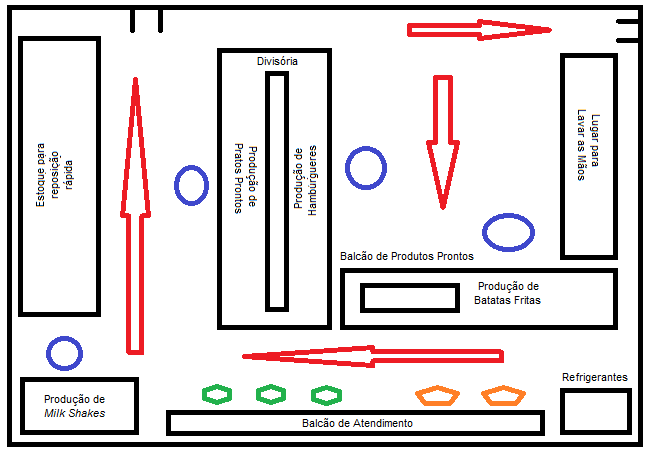
\includegraphics[scale=0.8]{arranjo3}
			\caption[Desenho esquemático do arranjo físico do Bob's no Taguatinga Shopping]{Desenho esquemático do arranjo físico do \textbf{Bob's} no \emph{Taguatinga Shopping}.}
			\label{fig:arranjo3}
		\end{figure}

		Legenda:
		\begin{figure}[h]
			\centering
			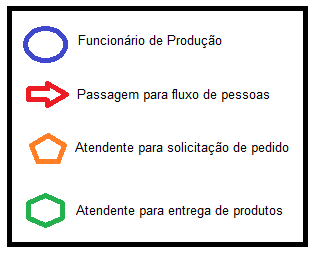
\includegraphics[scale=0.7]{arranjo4}
			\label{fig:arranjo4}
		\end{figure}

		É possível perceber que é uma estrutura física pequena, mas que aproveita o máximo de seu espaço, explorando todos os recursos físicos possíveis. Foram identificadas duas salas, uma para guarda parte do estoque e outra como departamento financeiro e de recursos humanos (ambas as salas não puderam ser vistas durante a visita). Os caminhos para fluxo de pessoas são bem estreitos, mas é possível a passagem sem muitas dificuldades.

		Como regras de negócio, a empresa trabalha com dois caixas de atendimento aos clientes para solicitação de pedidos, no qual segundo o gerente, é suficiente para a demanda de cliente. Também existem três caixas de atendimento para saída de produtos prontos, ou seja, entrega dos produtos solicitados pelos clientes. Essa quantia é suficiente, pois algumas das vezes é necessário a ajuda de um funcionário para o oferecimento de um serviço ao cliente, como por exemplo, a entrega de novos talheres.

		Os setores de produção são pequenos, cabendo apenas um funcionário, por este motivo, ainda existe um segundo funcionário que repõe o estoque quando solicitado. Os funcionários de produção normalmente possuem um treinamento especifico para produção extremamente rápida dos produtos. 
	
		Nas divisórias são acopladas prateleiras onde se encontrados os recursos a serem transformados. Tais como pães, queijos, hambúrgueres fritos, papeis filmes, saladas entre outros. Existem duas espécies de estoque, uma funciona como um depositório de produtos inorgânicos como copos, pratos, talheres e alguns orgânicos como leite, potes de milho e ervilha. E também existe o estoque rápido no qual todas as manhãs é realimentado. Ele serve para reposição rápida sem a necessidade de ir ao deposito recolher os produtos, isso facilita durante o período de produção, pois evita o congestionamento dos produtos durante o processo.

		É importante ressaltar que essa estrutura pode sofrer variáveis de acordo com o espaço físico disponível, isso foi um ponto importante abordado pelo gerente da franquia durante a entrevista. Outro ponto importante é que, atualmente o \textbf{Bob’s} possui essa estrutura padrão para a maioria das franquias, no entanto, uma mudança anunciada para os próximos anos, prevê uma modernização no design e infraestrutura operacional das lojas. Isso significa que possíveis mudanças no arranjo físico podem vir a ocorrer nesse processo de reestruturação.